\documentclass[tikz,border=8pt]{standalone}
% Shared look for every TikZ diagram. Load with \input{../../tools/tikz-style.tex}
\usepackage[T1]{fontenc}
\usepackage{lmodern}
\renewcommand{\sfdefault}{lmr}  % diagrams use the same serif as the text
\usetikzlibrary{arrows.meta, positioning, shapes.geometric, calc, fit, backgrounds}
\definecolor{cblue}{HTML}{4C78A8}
\definecolor{corange}{HTML}{F58518}
\definecolor{cgreen}{HTML}{54A24B}
\definecolor{cred}{HTML}{E45756}
\definecolor{cpurple}{HTML}{B279A2}
\definecolor{cgrey}{HTML}{6B6B6B}
\tikzset{
  every picture/.style={font=\sffamily, line width=1.2pt},
  box/.style={draw=#1, fill=#1!12, rounded corners=4pt, align=center, inner sep=7pt, minimum height=1.1cm},
  box/.default=cgrey,
  arrow/.style={-{Stealth[length=3mm]}, draw=cgrey, line width=1.4pt},
  title/.style={font=\sffamily\bfseries\Large},
  note/.style={font=\sffamily\small, text=cgrey, align=center},
}
\AtBeginDocument{\hyphenpenalty=10000 \exhyphenpenalty=10000}

\begin{document}
% Sections 4.4 and 4.5: the first three training sequences padded in front to 51 integers, then split into the
% input X (the first 50 columns) and the output y (the last column). Integers from section 4.2.
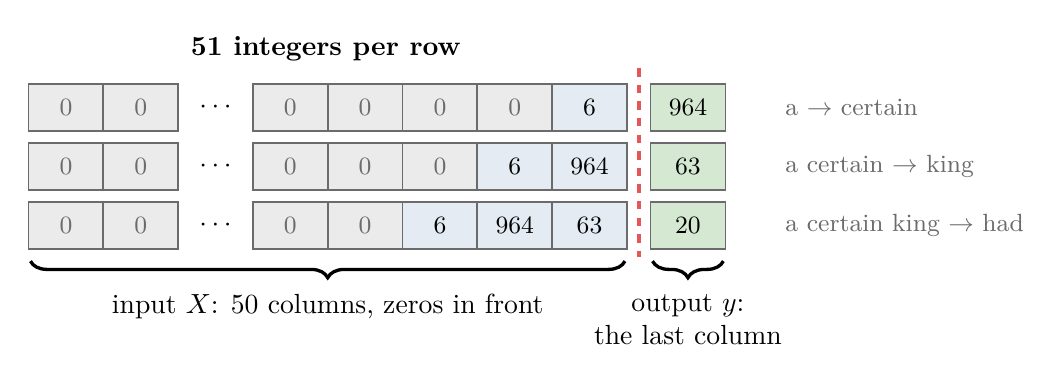
\begin{tikzpicture}[c/.style={draw=cgrey, minimum width=0.95cm, minimum height=0.6cm, font=\sffamily\small, line width=0.6pt},
                    zc/.style={c, fill=black!8, text=cgrey}, wc/.style={c, fill=cblue!15}, oc/.style={c, fill=cgreen!25}]
  \foreach \r/\lab in {0/{a $\to$ certain}, 1/{a certain $\to$ king}, 2/{a certain king $\to$ had}} {
    \node[zc] at (0, -\r*0.75) {0};
    \node[zc] at (0.95, -\r*0.75) {0};
    \node at (1.9, -\r*0.75) {$\cdots$};
    \node[zc] at (2.85, -\r*0.75) {0};
    \node[note, anchor=west] at (9.0, -\r*0.75) {\lab};
  }
  % row 0: 49 zeros, then 6 | 964
  \node[zc] at (3.8, 0) {0}; \node[zc] at (4.75, 0) {0}; \node[zc] at (5.7, 0) {0}; \node[wc] at (6.65, 0) {6}; \node[oc] at (7.9, 0) {964};
  % row 1: 48 zeros, then 6, 964 | 63
  \node[zc] at (3.8, -0.75) {0}; \node[zc] at (4.75, -0.75) {0}; \node[wc] at (5.7, -0.75) {6}; \node[wc] at (6.65, -0.75) {964}; \node[oc] at (7.9, -0.75) {63};
  % row 2: 47 zeros, then 6, 964, 63 | 20
  \node[zc] at (3.8, -1.5) {0}; \node[wc] at (4.75, -1.5) {6}; \node[wc] at (5.7, -1.5) {964}; \node[wc] at (6.65, -1.5) {63}; \node[oc] at (7.9, -1.5) {20};
  \draw[decorate, decoration={brace, amplitude=6pt, mirror}] (-0.45, -1.95) -- (7.1, -1.95)
    node[midway, below=8pt, font=\sffamily] {input $X$: 50 columns, zeros in front};
  \draw[decorate, decoration={brace, amplitude=6pt, mirror}] (7.45, -1.95) -- (8.35, -1.95)
    node[midway, below=8pt, font=\sffamily, align=center] {output $y$:\\the last column};
  \draw[cred, dashed, line width=1.2pt] (7.28, 0.5) -- (7.28, -1.9);
  \node[font=\sffamily\bfseries, anchor=south] at (3.3, 0.45) {51 integers per row};
\end{tikzpicture}
\end{document}
